% Options for packages loaded elsewhere
\PassOptionsToPackage{unicode}{hyperref}
\PassOptionsToPackage{hyphens}{url}
\PassOptionsToPackage{dvipsnames,svgnames,x11names}{xcolor}
%
\documentclass[
  letterpaper,
  DIV=11,
  numbers=noendperiod]{scrartcl}

\usepackage{amsmath,amssymb}
\usepackage{iftex}
\ifPDFTeX
  \usepackage[T1]{fontenc}
  \usepackage[utf8]{inputenc}
  \usepackage{textcomp} % provide euro and other symbols
\else % if luatex or xetex
  \usepackage{unicode-math}
  \defaultfontfeatures{Scale=MatchLowercase}
  \defaultfontfeatures[\rmfamily]{Ligatures=TeX,Scale=1}
\fi
\usepackage{lmodern}
\ifPDFTeX\else  
    % xetex/luatex font selection
\fi
% Use upquote if available, for straight quotes in verbatim environments
\IfFileExists{upquote.sty}{\usepackage{upquote}}{}
\IfFileExists{microtype.sty}{% use microtype if available
  \usepackage[]{microtype}
  \UseMicrotypeSet[protrusion]{basicmath} % disable protrusion for tt fonts
}{}
\makeatletter
\@ifundefined{KOMAClassName}{% if non-KOMA class
  \IfFileExists{parskip.sty}{%
    \usepackage{parskip}
  }{% else
    \setlength{\parindent}{0pt}
    \setlength{\parskip}{6pt plus 2pt minus 1pt}}
}{% if KOMA class
  \KOMAoptions{parskip=half}}
\makeatother
\usepackage{xcolor}
\setlength{\emergencystretch}{3em} % prevent overfull lines
\setcounter{secnumdepth}{-\maxdimen} % remove section numbering
% Make \paragraph and \subparagraph free-standing
\makeatletter
\ifx\paragraph\undefined\else
  \let\oldparagraph\paragraph
  \renewcommand{\paragraph}{
    \@ifstar
      \xxxParagraphStar
      \xxxParagraphNoStar
  }
  \newcommand{\xxxParagraphStar}[1]{\oldparagraph*{#1}\mbox{}}
  \newcommand{\xxxParagraphNoStar}[1]{\oldparagraph{#1}\mbox{}}
\fi
\ifx\subparagraph\undefined\else
  \let\oldsubparagraph\subparagraph
  \renewcommand{\subparagraph}{
    \@ifstar
      \xxxSubParagraphStar
      \xxxSubParagraphNoStar
  }
  \newcommand{\xxxSubParagraphStar}[1]{\oldsubparagraph*{#1}\mbox{}}
  \newcommand{\xxxSubParagraphNoStar}[1]{\oldsubparagraph{#1}\mbox{}}
\fi
\makeatother

\usepackage{color}
\usepackage{fancyvrb}
\newcommand{\VerbBar}{|}
\newcommand{\VERB}{\Verb[commandchars=\\\{\}]}
\DefineVerbatimEnvironment{Highlighting}{Verbatim}{commandchars=\\\{\}}
% Add ',fontsize=\small' for more characters per line
\usepackage{framed}
\definecolor{shadecolor}{RGB}{36,41,46}
\newenvironment{Shaded}{\begin{snugshade}}{\end{snugshade}}
\newcommand{\AlertTok}[1]{\textcolor[rgb]{1.00,0.33,0.33}{\textbf{#1}}}
\newcommand{\AnnotationTok}[1]{\textcolor[rgb]{0.42,0.45,0.49}{#1}}
\newcommand{\AttributeTok}[1]{\textcolor[rgb]{0.98,0.46,0.51}{#1}}
\newcommand{\BaseNTok}[1]{\textcolor[rgb]{0.47,0.72,1.00}{#1}}
\newcommand{\BuiltInTok}[1]{\textcolor[rgb]{0.98,0.46,0.51}{#1}}
\newcommand{\CharTok}[1]{\textcolor[rgb]{0.62,0.80,1.00}{#1}}
\newcommand{\CommentTok}[1]{\textcolor[rgb]{0.42,0.45,0.49}{#1}}
\newcommand{\CommentVarTok}[1]{\textcolor[rgb]{0.42,0.45,0.49}{#1}}
\newcommand{\ConstantTok}[1]{\textcolor[rgb]{0.47,0.72,1.00}{#1}}
\newcommand{\ControlFlowTok}[1]{\textcolor[rgb]{0.98,0.46,0.51}{#1}}
\newcommand{\DataTypeTok}[1]{\textcolor[rgb]{0.98,0.46,0.51}{#1}}
\newcommand{\DecValTok}[1]{\textcolor[rgb]{0.47,0.72,1.00}{#1}}
\newcommand{\DocumentationTok}[1]{\textcolor[rgb]{0.42,0.45,0.49}{#1}}
\newcommand{\ErrorTok}[1]{\textcolor[rgb]{1.00,0.33,0.33}{\underline{#1}}}
\newcommand{\ExtensionTok}[1]{\textcolor[rgb]{0.98,0.46,0.51}{\textbf{#1}}}
\newcommand{\FloatTok}[1]{\textcolor[rgb]{0.47,0.72,1.00}{#1}}
\newcommand{\FunctionTok}[1]{\textcolor[rgb]{0.70,0.57,0.94}{#1}}
\newcommand{\ImportTok}[1]{\textcolor[rgb]{0.62,0.80,1.00}{#1}}
\newcommand{\InformationTok}[1]{\textcolor[rgb]{0.42,0.45,0.49}{#1}}
\newcommand{\KeywordTok}[1]{\textcolor[rgb]{0.98,0.46,0.51}{#1}}
\newcommand{\NormalTok}[1]{\textcolor[rgb]{0.88,0.89,0.91}{#1}}
\newcommand{\OperatorTok}[1]{\textcolor[rgb]{0.88,0.89,0.91}{#1}}
\newcommand{\OtherTok}[1]{\textcolor[rgb]{0.70,0.57,0.94}{#1}}
\newcommand{\PreprocessorTok}[1]{\textcolor[rgb]{0.98,0.46,0.51}{#1}}
\newcommand{\RegionMarkerTok}[1]{\textcolor[rgb]{0.42,0.45,0.49}{#1}}
\newcommand{\SpecialCharTok}[1]{\textcolor[rgb]{0.47,0.72,1.00}{#1}}
\newcommand{\SpecialStringTok}[1]{\textcolor[rgb]{0.62,0.80,1.00}{#1}}
\newcommand{\StringTok}[1]{\textcolor[rgb]{0.62,0.80,1.00}{#1}}
\newcommand{\VariableTok}[1]{\textcolor[rgb]{1.00,0.67,0.44}{#1}}
\newcommand{\VerbatimStringTok}[1]{\textcolor[rgb]{0.62,0.80,1.00}{#1}}
\newcommand{\WarningTok}[1]{\textcolor[rgb]{1.00,0.33,0.33}{#1}}

\providecommand{\tightlist}{%
  \setlength{\itemsep}{0pt}\setlength{\parskip}{0pt}}\usepackage{longtable,booktabs,array}
\usepackage{calc} % for calculating minipage widths
% Correct order of tables after \paragraph or \subparagraph
\usepackage{etoolbox}
\makeatletter
\patchcmd\longtable{\par}{\if@noskipsec\mbox{}\fi\par}{}{}
\makeatother
% Allow footnotes in longtable head/foot
\IfFileExists{footnotehyper.sty}{\usepackage{footnotehyper}}{\usepackage{footnote}}
\makesavenoteenv{longtable}
\usepackage{graphicx}
\makeatletter
\newsavebox\pandoc@box
\newcommand*\pandocbounded[1]{% scales image to fit in text height/width
  \sbox\pandoc@box{#1}%
  \Gscale@div\@tempa{\textheight}{\dimexpr\ht\pandoc@box+\dp\pandoc@box\relax}%
  \Gscale@div\@tempb{\linewidth}{\wd\pandoc@box}%
  \ifdim\@tempb\p@<\@tempa\p@\let\@tempa\@tempb\fi% select the smaller of both
  \ifdim\@tempa\p@<\p@\scalebox{\@tempa}{\usebox\pandoc@box}%
  \else\usebox{\pandoc@box}%
  \fi%
}
% Set default figure placement to htbp
\def\fps@figure{htbp}
\makeatother

% Load packages
\usepackage{geometry} % For setting page dimensions
\usepackage{xcolor} % For defining and using colors
\usepackage{eso-pic} % For adding elements to each page
\usepackage{fancyhdr} % For custom page headers and footers
\usepackage{sectsty} % For styling section and chapter titles
\usepackage{titlesec} % For customizing section titles
\usepackage{listings} % For including code listings
\usepackage{setspace} % For adjusting line spacing
\usepackage{mfirstuc}

% Define colors
\definecolor{light}{HTML}{000000}
\definecolor{highlight}{HTML}{800080}
\definecolor{dark}{HTML}{330033}


% Define page setup variables for letter size
\newcommand{\mypapersize}{letterpaper} % Change from a4paper to letterpaper
\newcommand{\mytotal}{215.9mm,279.4mm} % Dimensions for letter size (8.5in x 11in in mm)
\newcommand{\myleft}{25mm} % You might want to adjust these margins as needed
\newcommand{\mytop}{15mm}
\newcommand{\mybottom}{25mm}
\newcommand{\myright}{35mm}

% Set page setup for letter size
\geometry{\mypapersize, total={\mytotal}, left=\myleft, top=\mytop, bottom=\mybottom, right=\myright}

% Title alignment with custom line spacing
\makeatletter
\renewcommand{\maketitle}{
    \bgroup
    \begin{flushleft}
        % Begin a spacing environment for the title section
        \begin{spacing}{1.25}
        {\sffamily\fontsize{25}{20}\textbf{\capitalisewords{\@title}}} \vspace{0.3cm} \newline
        {\large\@author} \newline
        {\large\today} \newline % Include the full date here
        {\large {\@subtitle}} \vspace{-1cm}
        \end{spacing} % End the spacing environment
    \end{flushleft}
    \egroup
}
\makeatother

% Set the main document line spacing to double
\setstretch{1.15} % Or \doublespacing

% Section styles
% Section font settings
\titleformat{\section}{\vspace{-0.5cm}\sffamily\fontsize{18}{20}\bfseries}{\thesection}{1.1em}{}[{\titlerule[2pt]}]
\titleformat{\subsection}{\sffamily\fontsize{15}{15}\bfseries}{\thesubsection}{1.1em}{}[{\titlerule[1pt]}]
\titleformat{\subsubsection}{\sffamily\fontsize{13}{13}\bfseries}{\thesubsubsection}{1.1em}{}[{\titlerule[0.5pt]}]

% Logo and bar placement
\AddToShipoutPicture{% 
    \AtPageLowerLeft{% 
        \put(\LenToUnit{\dimexpr\paperwidth-2.75cm},25cm){% 
            \color{light}\rule{3.25cm}{3cm}% Adjust the height as needed
        }%
    }%
    \AtPageLowerLeft{% start the bar at the bottom right of the page
        \put(\LenToUnit{\dimexpr\paperwidth-2.6cm},25.2cm){% move it to the top right
            \color{light}
\includegraphics[width=2.5cm]{_extensions/OSULatexTheme/logo.png}
        }%
    }%
}

% Other Page Styling
\fancypagestyle{mystyle}{
  \fancyhf{}
  \renewcommand\headrulewidth{0pt}
  \fancyfoot[R]{\fontsize{20}{12}\selectfont\thepage} 
  \fancyfootoffset{2cm}
  \setlength{\footskip}{20pt}
}



\pagestyle{mystyle}
\usepackage{fvextra}
\DefineVerbatimEnvironment{Highlighting}{Verbatim}{breaklines,commandchars=\\\{\}}
\KOMAoption{captions}{tableheading}
\makeatletter
\@ifpackageloaded{caption}{}{\usepackage{caption}}
\AtBeginDocument{%
\ifdefined\contentsname
  \renewcommand*\contentsname{Table of contents}
\else
  \newcommand\contentsname{Table of contents}
\fi
\ifdefined\listfigurename
  \renewcommand*\listfigurename{List of Figures}
\else
  \newcommand\listfigurename{List of Figures}
\fi
\ifdefined\listtablename
  \renewcommand*\listtablename{List of Tables}
\else
  \newcommand\listtablename{List of Tables}
\fi
\ifdefined\figurename
  \renewcommand*\figurename{Figure}
\else
  \newcommand\figurename{Figure}
\fi
\ifdefined\tablename
  \renewcommand*\tablename{Table}
\else
  \newcommand\tablename{Table}
\fi
}
\@ifpackageloaded{float}{}{\usepackage{float}}
\floatstyle{ruled}
\@ifundefined{c@chapter}{\newfloat{codelisting}{h}{lop}}{\newfloat{codelisting}{h}{lop}[chapter]}
\floatname{codelisting}{Listing}
\newcommand*\listoflistings{\listof{codelisting}{List of Listings}}
\makeatother
\makeatletter
\makeatother
\makeatletter
\@ifpackageloaded{caption}{}{\usepackage{caption}}
\@ifpackageloaded{subcaption}{}{\usepackage{subcaption}}
\makeatother
\makeatletter
\@ifpackageloaded{tcolorbox}{}{\usepackage[skins,breakable]{tcolorbox}}
\makeatother
\makeatletter
\@ifundefined{shadecolor}{\definecolor{shadecolor}{rgb}{.97, .97, .97}}{}
\makeatother
\makeatletter
\@ifundefined{codebgcolor}{\definecolor{codebgcolor}{HTML}{000000}}{}
\makeatother
\makeatletter
\ifdefined\Shaded\renewenvironment{Shaded}{\begin{tcolorbox}[colback={codebgcolor}, frame hidden, breakable, boxrule=0pt, sharp corners, enhanced]}{\end{tcolorbox}}\fi
\makeatother

\usepackage{bookmark}

\IfFileExists{xurl.sty}{\usepackage{xurl}}{} % add URL line breaks if available
\urlstyle{same} % disable monospaced font for URLs
\hypersetup{
  pdftitle={Final Project Report: Bar Crawl Heavy Drinking},
  pdfauthor={Brian Cervantes Alvarez},
  colorlinks=true,
  linkcolor={highlight},
  filecolor={Maroon},
  citecolor={Blue},
  urlcolor={highlight},
  pdfcreator={LaTeX via pandoc}}


\title{Final Project Report: Bar Crawl Heavy Drinking}
\author{Brian Cervantes Alvarez}
\date{Monday, March 17, 2025}

\begin{document}
\maketitle

\pagestyle{mystyle}


\section{Introduction}\label{introduction}

The goal of this final project is to demonstrate proficiency in working
with a \textbf{very large dataset} across \textbf{multiple tools},
primarily \textbf{Apache Spark} on Google Dataproc and \textbf{Google
Cloud Storage} (GCS). I selected the \textbf{Bar Crawl: Detecting Heavy
Drinking} dataset, which contains:

\begin{itemize}
\tightlist
\item
  \textbf{Accelerometer readings} (over 14 million rows) from 13
  participants.
\item
  \textbf{Transdermal Alcohol Content (TAC)} readings collected at
  30-minute intervals.
\item
  \textbf{Phone type} metadata (iPhone vs.~Android).
\item
  \textbf{Time-aligned} data for each participant, used to study heavy
  drinking patterns.
\end{itemize}

\subsection{Statement of Originality}\label{statement-of-originality}

I worked on this project by myself. During the programming phase, I
received coding assistance and suggestions for error handling from
GitHub Copilot and ChatGPT for full transparency. However, all final
analysis, code, and documentation in this report are my own.

\subsection{Data \& Complexity}\label{data-complexity}

This
\href{https://archive.ics.uci.edu/dataset/515/bar+crawl+detecting+heavy+drinking}{dataset}
meets several complexity criteria:

\begin{itemize}
\tightlist
\item
  \textbf{Data not standardized}: We merged multiple CSV files
  (accelerometer data, phone types, TAC readings).
\item
  \textbf{Split across multiple files}: The original dataset included
  many CSVs, plus separate TAC files.
\item
  \textbf{Contains strings with punctuation}: For example, phone type
  CSV includes text fields.
\item
  \textbf{Larger than 1GB}: After merging, the dataset is about 1.5 GB.
\item
  \textbf{Multiple data types}: Time series, numeric, string.
\item
  \textbf{Access method}: I uploaded the merged dataset to
  \textbf{Google Cloud Storage} (GCS) and processed it with
  \textbf{Spark} on a Dataproc cluster.
\end{itemize}

By the rubric's scoring, it easily exceeds the \textbf{5--7 points}
threshold for a suitably challenging dataset.

\section{OSEMN Process}\label{osemn-process}

I loosely followed the \textbf{OSEMN} steps: \textbf{Obtain, Scrub,
Explore, Model, iNterpret}.

\begin{enumerate}
\def\labelenumi{\arabic{enumi}.}
\tightlist
\item
  \textbf{Obtain}: Downloaded raw accelerometer CSV
  (\texttt{all\_accelerometer\_data\_pids\_13.csv}), phone types, and
  TAC data from the official repository.
\item
  \textbf{Scrub}:

  \begin{itemize}
  \tightlist
  \item
    Merged phone types by \texttt{pid}.
  \item
    Cleaned TAC data to remove unusable participants.
  \item
    Time-aligned each accelerometer row with the nearest TAC reading
    using Pandas' \texttt{merge\_asof}.
  \end{itemize}
\item
  \textbf{Explore}:

  \begin{itemize}
  \tightlist
  \item
    Investigated distributions of \texttt{(x,\ y,\ z)} by phone type.
  \item
    Computed correlation between magnitude and TAC.
  \end{itemize}
\item
  \textbf{Model}:

  \begin{itemize}
  \tightlist
  \item
    K-means clustering on \texttt{(x,\ y,\ z,\ magnitude)}.
  \item
    Logistic regression to predict heavy drinking (TAC \textgreater=
    0.08).
  \end{itemize}
\item
  \textbf{iNterpret}:

  \begin{itemize}
  \tightlist
  \item
    Visualized cluster results (PCA 2D).
  \item
    Examined logistic regression performance (AUC ≈ 0.52--0.57).
  \end{itemize}
\end{enumerate}

\section{Loading \& Big Data Tools}\label{loading-big-data-tools}

\subsection{Google Cloud Storage (GCS)}\label{google-cloud-storage-gcs}

\begin{enumerate}
\def\labelenumi{\arabic{enumi}.}
\tightlist
\item
  I uploaded the merged CSV (time\_aligned\_barCrawl.csv) to
  \textbf{GCS}.
\item
  Used \texttt{gsutil} to verify the file was in the bucket.
\item
  Spark read the file directly from
  \texttt{gs://ds512\_drinking\_data/time\_aligned\_barCrawl.csv}.
\end{enumerate}

\subsection{Spark (Dataproc)}\label{spark-dataproc}

\begin{enumerate}
\def\labelenumi{\arabic{enumi}.}
\tightlist
\item
  Created a Dataproc cluster with enough memory to handle
  \textasciitilde1.5 GB of data.
\item
  Used Spark DataFrames to:

  \begin{itemize}
  \tightlist
  \item
    Compute time window stats (group by 1-minute windows).
  \item
    Run K-means clustering.
  \item
    Run logistic regression (with cross-validation).
  \end{itemize}
\item
  Wrote results (CSVs) and saved plots to GCS.
\end{enumerate}

\section{Three Questions}\label{three-questions}

\textbf{Q1: Does phone type (iPhone vs.~Android) affect average
accelerometer readings?}\\
- Grouped by \texttt{phonetype} and computed
\texttt{(avg\_x,\ std\_x,\ avg\_y,\ std\_y,\ avg\_z,\ std\_z)}.\\
- \textbf{Result}: iPhones had near-zero averages. Android had a large
offset in \texttt{y} and \texttt{z}, likely from sensor calibration
differences.

\textbf{Q2: How does acceleration magnitude vary over time, and is it
correlated with TAC?}\\
- Computed magnitude = \(\sqrt{x^2 + y^2 + z^2}\).\\
- Grouped into 1-minute windows =\textgreater{} average magnitude.\\
- Correlation with TAC\_Reading is about 0.0489, extremely low.

\textbf{Q3: Can we predict intoxication (TAC \textgreater= 0.08) using
\texttt{(x,\ y,\ z,\ magnitude)}?}\\
- Used a \textbf{scaled-down logistic regression} with
cross-validation.\\
- Achieved an AUC of \textasciitilde0.52--0.57, which indicates a weak
predictive signal from just these raw features.

\section{Visualizations \& Findings}\label{visualizations-findings}

\begin{enumerate}
\def\labelenumi{\arabic{enumi}.}
\item
  \textbf{Phone Type Boxplots}\\
  \pandocbounded{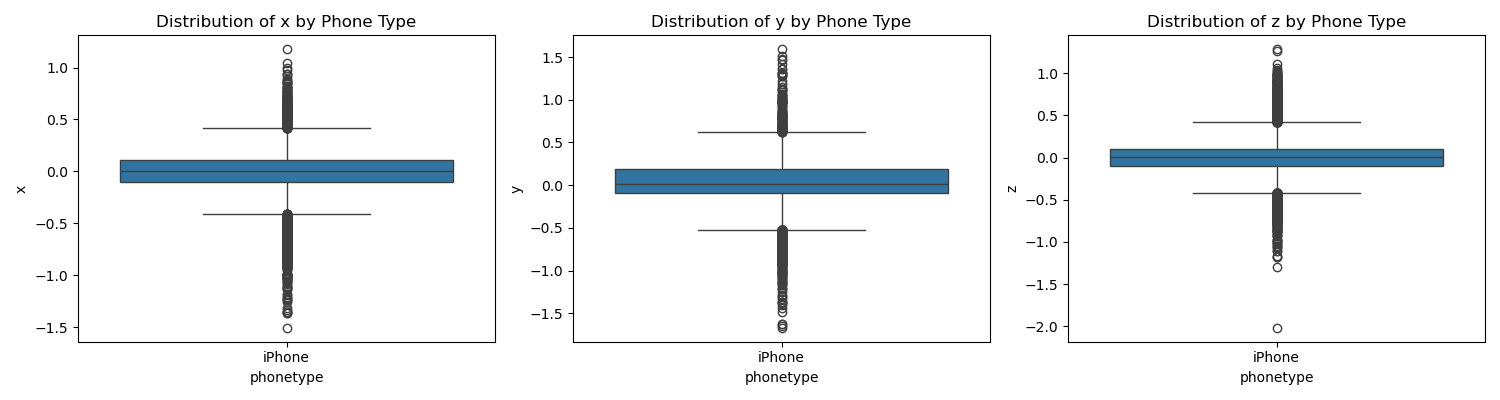
\includegraphics[keepaspectratio]{phone_boxplots.png}}
\item
  \textbf{Temporal Patterns}\\
  \pandocbounded{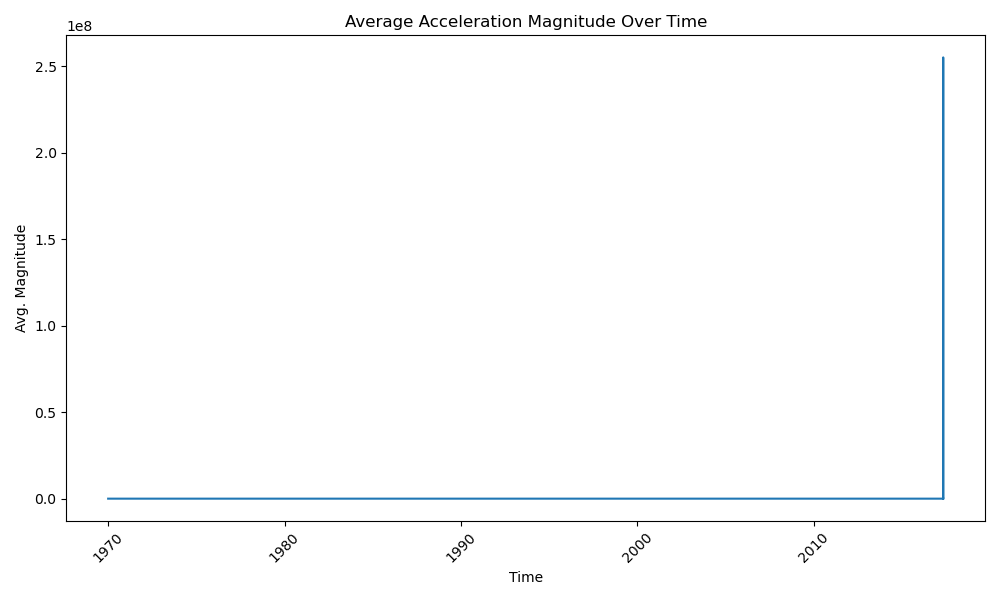
\includegraphics[keepaspectratio]{avg_magnitude_timeseries.png}}\\
  Some participants produce huge outlier readings, causing a large
  spike.
\item
  \textbf{K-means Clustering}\\
  \pandocbounded{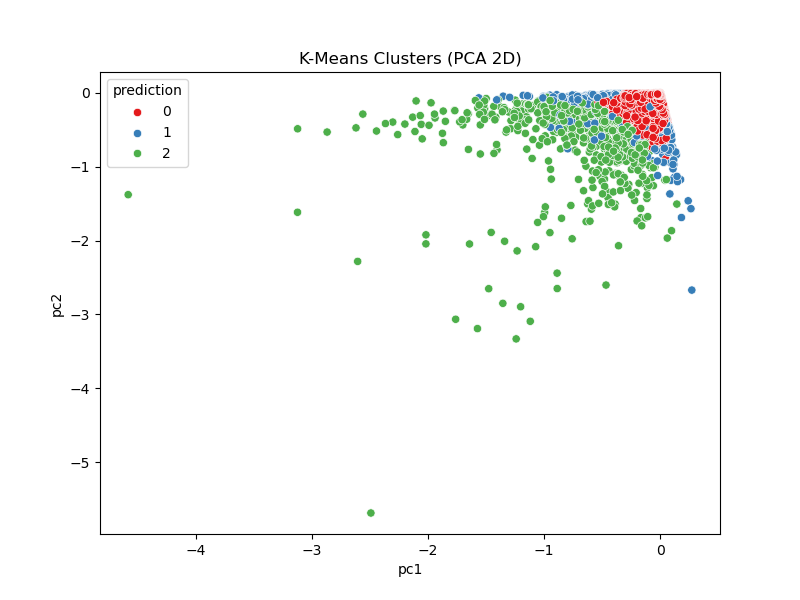
\includegraphics[keepaspectratio]{kmeans_pca.png}}\\
  Clusters are somewhat distinct, though overshadowed by outliers.
\item
  \textbf{Correlation}\\
  \pandocbounded{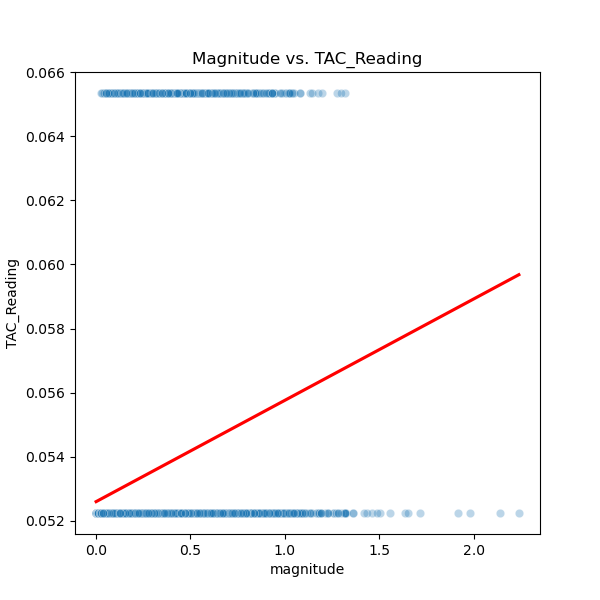
\includegraphics[keepaspectratio]{magnitude_TAC_scatter.png}}\\
  Very weak correlation (≈0.05) between magnitude \& TAC.
\item
  \textbf{ROC Curve}\\
  \pandocbounded{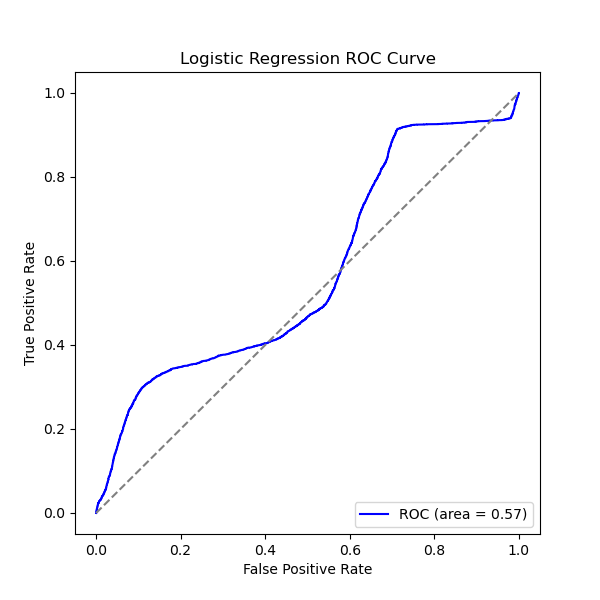
\includegraphics[keepaspectratio]{lr_roc_curve.png}}\\
  AUC \textasciitilde0.52--0.57, which is barely above random guessing.
\end{enumerate}

\section{Conclusion \& Reflection}\label{conclusion-reflection}

\begin{itemize}
\tightlist
\item
  \textbf{Dataset Size}: \textasciitilde1.5 GB after merging, so
  distributed computing was necessary.
\item
  \textbf{Observations}:

  \begin{itemize}
  \tightlist
  \item
    A large numeric offset for Android data implies a sensor calibration
    issue.
  \item
    Correlation between magnitude \& TAC is nearly zero, consistent with
    the low logistic regression AUC.
  \end{itemize}
\item
  \textbf{Future Work}:

  \begin{itemize}
  \tightlist
  \item
    Incorporate \textbf{window-based feature engineering} (e.g.,
    standard deviation or spectral features).
  \item
    Gather additional phone usage context to improve intoxication
    predictions.
  \end{itemize}
\end{itemize}

\section{References}\label{references}

\begin{itemize}
\tightlist
\item
  Killian, J.A., Passino, K.M., Nandi, A., Madden, D.R. and Clapp, J.
  \emph{Learning to Detect Heavy Drinking Episodes Using Smartphone
  Accelerometer Data.} In \textbf{Proceedings of the 4th International
  Workshop on Knowledge Discovery in Healthcare Data} co-located with
  the 28th International Joint Conference on Artificial Intelligence
  (IJCAI 2019) (pp.~35-42). \url{http://ceur-ws.org/Vol-2429/paper6.pdf}
\end{itemize}

\section{Appendix}\label{appendix}

\subsection{PySpark Script}\label{pyspark-script}

Below is the PySpark script (\texttt{barCrawlAnalysis.py}) that runs on
Google Dataproc. We read from
\texttt{gs://ds512\_drinking\_data/time\_aligned\_barCrawl.csv}, perform
the analyses, and write results + plots to GCS. Comments, error-handling
and partial code suggestions were assisted by Copilot \& ChatGPT.

\begin{Shaded}
\begin{Highlighting}[]
\CommentTok{\#!/usr/bin/env python3}
\CommentTok{"""}
\CommentTok{Enhanced PySpark Script for Bar Crawl Heavy Drinking Data Analysis}
\CommentTok{Saving CSV outputs and plots to GCS.}

\CommentTok{DATASET ORIGINS:}
\CommentTok{    We obtained "time\_aligned\_barCrawl.csv" by:}
\CommentTok{      1) Merging "all\_accelerometer\_data\_pids\_13.csv" with phone\_types.csv by pid.}
\CommentTok{      2) For each participant, reading their "clean\_tac/*.csv" file (with columns timestamp, TAC\_Reading).}
\CommentTok{      3) Converting both timestamps to comparable datetime formats.}
\CommentTok{      4) Using Pandas\textquotesingle{} merge\_asof (nearest join) to time{-}align each accelerometer row to the closest TAC reading.}
\CommentTok{      5) Concatenating all participants into one final CSV, renamed "time\_aligned\_barCrawl.csv".}

\CommentTok{SCRIPT STEPS:}
\CommentTok{    1. Reads "time\_aligned\_barCrawl.csv" from GCS into Spark.}
\CommentTok{    2. Analysis 1: Phone type impact on accelerometer readings.}
\CommentTok{    3. Analysis 2: Temporal patterns (compute magnitude, group by 1{-}minute windows).}
\CommentTok{    4. Analysis 3: K{-}means clustering on a sample of accelerometer data (with a PCA figure).}
\CommentTok{    5. Analysis 4: Correlation between magnitude and TAC\_Reading (with a scatter plot).}
\CommentTok{    6. Analysis 5: Scaled{-}Down Logistic Regression (using cross{-}validation with a limited grid and sample)}
\CommentTok{       to predict intoxication (TAC \textgreater{}= 0.08).}
\CommentTok{    7. Writes CSV results to GCS. Plots are saved locally, then uploaded to GCS.}

\CommentTok{Run:}
\CommentTok{  gsutil {-}m cp {-}r "gs://ds512\_drinking\_data/results" .}
\CommentTok{to download the /results folder from GCS to your local machine.}
\CommentTok{"""}

\ImportTok{import}\NormalTok{ os}
\ImportTok{import}\NormalTok{ pyspark}
\ImportTok{from}\NormalTok{ pyspark.sql }\ImportTok{import}\NormalTok{ SparkSession}
\ImportTok{from}\NormalTok{ pyspark.sql.functions }\ImportTok{import}\NormalTok{ (}
\NormalTok{    avg, stddev, sqrt, col, from\_unixtime, window, when, corr}
\NormalTok{)}
\ImportTok{from}\NormalTok{ pyspark.ml.feature }\ImportTok{import}\NormalTok{ VectorAssembler}
\ImportTok{from}\NormalTok{ pyspark.ml.clustering }\ImportTok{import}\NormalTok{ KMeans}
\ImportTok{from}\NormalTok{ pyspark.ml.classification }\ImportTok{import}\NormalTok{ LogisticRegression}
\ImportTok{from}\NormalTok{ pyspark.ml.evaluation }\ImportTok{import}\NormalTok{ BinaryClassificationEvaluator}
\ImportTok{from}\NormalTok{ pyspark.ml.tuning }\ImportTok{import}\NormalTok{ ParamGridBuilder, CrossValidator}

\ImportTok{import}\NormalTok{ matplotlib}
\NormalTok{matplotlib.use(}\StringTok{\textquotesingle{}Agg\textquotesingle{}}\NormalTok{)}
\ImportTok{import}\NormalTok{ matplotlib.pyplot }\ImportTok{as}\NormalTok{ plt}
\ImportTok{import}\NormalTok{ seaborn }\ImportTok{as}\NormalTok{ sns}

\CommentTok{\# For uploading images to GCS}
\ImportTok{from}\NormalTok{ google.cloud }\ImportTok{import}\NormalTok{ storage}

\KeywordTok{def}\NormalTok{ upload\_file\_to\_gcs(local\_path, bucket\_name, gcs\_path):}
    \CommentTok{"""}
\CommentTok{    Uploads a local file to a GCS path using the google{-}cloud{-}storage library.}
\CommentTok{    Example gcs\_path: \textquotesingle{}results/analysis1\_phone\_type/phone\_boxplots.png\textquotesingle{}}
\CommentTok{    """}
\NormalTok{    client }\OperatorTok{=}\NormalTok{ storage.Client()}
\NormalTok{    bucket }\OperatorTok{=}\NormalTok{ client.bucket(bucket\_name)}
\NormalTok{    blob }\OperatorTok{=}\NormalTok{ bucket.blob(gcs\_path)}
\NormalTok{    blob.upload\_from\_filename(local\_path)}
    \BuiltInTok{print}\NormalTok{(}\SpecialStringTok{f"Uploaded }\SpecialCharTok{\{}\NormalTok{local\_path}\SpecialCharTok{\}}\SpecialStringTok{ to gs://}\SpecialCharTok{\{}\NormalTok{bucket\_name}\SpecialCharTok{\}}\SpecialStringTok{/}\SpecialCharTok{\{}\NormalTok{gcs\_path}\SpecialCharTok{\}}\SpecialStringTok{"}\NormalTok{)}

\KeywordTok{def}\NormalTok{ main():}
\NormalTok{    spark }\OperatorTok{=}\NormalTok{ SparkSession.builder }\OperatorTok{\textbackslash{}}
\NormalTok{        .appName(}\StringTok{"barCrawlAnalysisToGCS"}\NormalTok{) }\OperatorTok{\textbackslash{}}
\NormalTok{        .master(}\StringTok{"yarn"}\NormalTok{) }\OperatorTok{\textbackslash{}}
\NormalTok{        .getOrCreate()}

\NormalTok{    bucket\_name }\OperatorTok{=} \StringTok{"ds512\_drinking\_data"}
\NormalTok{    base\_gcs\_path }\OperatorTok{=} \StringTok{"results"}

\NormalTok{    dataset\_path }\OperatorTok{=} \StringTok{"gs://ds512\_drinking\_data/time\_aligned\_barCrawl.csv"}
    \BuiltInTok{print}\NormalTok{(}\SpecialStringTok{f"Reading dataset from }\SpecialCharTok{\{}\NormalTok{dataset\_path}\SpecialCharTok{\}}\SpecialStringTok{..."}\NormalTok{)}
\NormalTok{    df }\OperatorTok{=}\NormalTok{ spark.read.}\BuiltInTok{format}\NormalTok{(}\StringTok{"csv"}\NormalTok{) }\OperatorTok{\textbackslash{}}
\NormalTok{        .option(}\StringTok{"header"}\NormalTok{, }\StringTok{"true"}\NormalTok{) }\OperatorTok{\textbackslash{}}
\NormalTok{        .option(}\StringTok{"inferSchema"}\NormalTok{, }\StringTok{"true"}\NormalTok{) }\OperatorTok{\textbackslash{}}
\NormalTok{        .load(dataset\_path)}

\NormalTok{    df }\OperatorTok{=}\NormalTok{ df.withColumn(}\StringTok{"time"}\NormalTok{, col(}\StringTok{"time"}\NormalTok{).cast(}\StringTok{"long"}\NormalTok{)) }\OperatorTok{\textbackslash{}}
\NormalTok{           .withColumn(}\StringTok{"x"}\NormalTok{, col(}\StringTok{"x"}\NormalTok{).cast(}\StringTok{"float"}\NormalTok{)) }\OperatorTok{\textbackslash{}}
\NormalTok{           .withColumn(}\StringTok{"y"}\NormalTok{, col(}\StringTok{"y"}\NormalTok{).cast(}\StringTok{"float"}\NormalTok{)) }\OperatorTok{\textbackslash{}}
\NormalTok{           .withColumn(}\StringTok{"z"}\NormalTok{, col(}\StringTok{"z"}\NormalTok{).cast(}\StringTok{"float"}\NormalTok{)) }\OperatorTok{\textbackslash{}}
\NormalTok{           .withColumn(}\StringTok{"TAC\_Reading"}\NormalTok{, col(}\StringTok{"TAC\_Reading"}\NormalTok{).cast(}\StringTok{"float"}\NormalTok{)) }\OperatorTok{\textbackslash{}}
\NormalTok{           .withColumn(}\StringTok{"datetime"}\NormalTok{, col(}\StringTok{"datetime"}\NormalTok{).cast(}\StringTok{"timestamp"}\NormalTok{))}

    \CommentTok{\# Analysis 1: Phone Type Impact}
\NormalTok{    phone\_stats }\OperatorTok{=}\NormalTok{ df.groupBy(}\StringTok{"phonetype"}\NormalTok{).agg(}
\NormalTok{        avg(}\StringTok{"x"}\NormalTok{).alias(}\StringTok{"avg\_x"}\NormalTok{),}
\NormalTok{        stddev(}\StringTok{"x"}\NormalTok{).alias(}\StringTok{"std\_x"}\NormalTok{),}
\NormalTok{        avg(}\StringTok{"y"}\NormalTok{).alias(}\StringTok{"avg\_y"}\NormalTok{),}
\NormalTok{        stddev(}\StringTok{"y"}\NormalTok{).alias(}\StringTok{"std\_y"}\NormalTok{),}
\NormalTok{        avg(}\StringTok{"z"}\NormalTok{).alias(}\StringTok{"avg\_z"}\NormalTok{),}
\NormalTok{        stddev(}\StringTok{"z"}\NormalTok{).alias(}\StringTok{"std\_z"}\NormalTok{)}
\NormalTok{    )}
\NormalTok{    phone\_stats.write.csv(}
        \SpecialStringTok{f"gs://}\SpecialCharTok{\{}\NormalTok{bucket\_name}\SpecialCharTok{\}}\SpecialStringTok{/}\SpecialCharTok{\{}\NormalTok{base\_gcs\_path}\SpecialCharTok{\}}\SpecialStringTok{/analysis1\_phone\_type/phone\_stats"}\NormalTok{,}
\NormalTok{        header}\OperatorTok{=}\VariableTok{True}\NormalTok{,}
\NormalTok{        mode}\OperatorTok{=}\StringTok{"overwrite"}
\NormalTok{    )}
    \BuiltInTok{print}\NormalTok{(}\StringTok{"Wrote phone\_stats to GCS (analysis1\_phone\_type)."}\NormalTok{)}

    \CommentTok{\# Analysis 2: Temporal Patterns}
\NormalTok{    df }\OperatorTok{=}\NormalTok{ df.withColumn(}\StringTok{"magnitude"}\NormalTok{, sqrt(col(}\StringTok{"x"}\NormalTok{)}\OperatorTok{**}\DecValTok{2} \OperatorTok{+}\NormalTok{ col(}\StringTok{"y"}\NormalTok{)}\OperatorTok{**}\DecValTok{2} \OperatorTok{+}\NormalTok{ col(}\StringTok{"z"}\NormalTok{)}\OperatorTok{**}\DecValTok{2}\NormalTok{))}
\NormalTok{    time\_window\_stats }\OperatorTok{=}\NormalTok{ df.groupBy(window(}\StringTok{"datetime"}\NormalTok{, }\StringTok{"1 minute"}\NormalTok{)).agg(}
\NormalTok{        avg(}\StringTok{"magnitude"}\NormalTok{).alias(}\StringTok{"avg\_magnitude"}\NormalTok{)}
\NormalTok{    )}
    \CommentTok{\# Flatten struct column}
\NormalTok{    time\_window\_stats\_flat }\OperatorTok{=}\NormalTok{ time\_window\_stats }\OperatorTok{\textbackslash{}}
\NormalTok{        .withColumn(}\StringTok{"window\_start"}\NormalTok{, col(}\StringTok{"window.start"}\NormalTok{)) }\OperatorTok{\textbackslash{}}
\NormalTok{        .withColumn(}\StringTok{"window\_end"}\NormalTok{, col(}\StringTok{"window.end"}\NormalTok{)) }\OperatorTok{\textbackslash{}}
\NormalTok{        .drop(}\StringTok{"window"}\NormalTok{)}

\NormalTok{    time\_window\_stats\_flat.write.csv(}
        \SpecialStringTok{f"gs://}\SpecialCharTok{\{}\NormalTok{bucket\_name}\SpecialCharTok{\}}\SpecialStringTok{/}\SpecialCharTok{\{}\NormalTok{base\_gcs\_path}\SpecialCharTok{\}}\SpecialStringTok{/analysis2\_temporal/time\_window\_stats"}\NormalTok{,}
\NormalTok{        header}\OperatorTok{=}\VariableTok{True}\NormalTok{,}
\NormalTok{        mode}\OperatorTok{=}\StringTok{"overwrite"}
\NormalTok{    )}
    \BuiltInTok{print}\NormalTok{(}\StringTok{"Wrote time\_window\_stats to GCS (analysis2\_temporal)."}\NormalTok{)}

    \CommentTok{\# Analysis 3: K{-}Means Clustering}
\NormalTok{    df\_sample }\OperatorTok{=}\NormalTok{ df.select(}\StringTok{"x"}\NormalTok{, }\StringTok{"y"}\NormalTok{, }\StringTok{"z"}\NormalTok{, }\StringTok{"magnitude"}\NormalTok{).limit(}\DecValTok{20000}\NormalTok{)}
\NormalTok{    assembler }\OperatorTok{=}\NormalTok{ VectorAssembler(inputCols}\OperatorTok{=}\NormalTok{[}\StringTok{"x"}\NormalTok{, }\StringTok{"y"}\NormalTok{, }\StringTok{"z"}\NormalTok{, }\StringTok{"magnitude"}\NormalTok{], outputCol}\OperatorTok{=}\StringTok{"features"}\NormalTok{)}
\NormalTok{    df\_features }\OperatorTok{=}\NormalTok{ assembler.transform(df\_sample).select(}\StringTok{"features"}\NormalTok{)}
\NormalTok{    kmeans }\OperatorTok{=}\NormalTok{ KMeans(k}\OperatorTok{=}\DecValTok{3}\NormalTok{, seed}\OperatorTok{=}\DecValTok{1}\NormalTok{)}
\NormalTok{    model }\OperatorTok{=}\NormalTok{ kmeans.fit(df\_features)}
\NormalTok{    predictions }\OperatorTok{=}\NormalTok{ model.transform(df\_features)}
\NormalTok{    cluster\_counts }\OperatorTok{=}\NormalTok{ predictions.groupBy(}\StringTok{"prediction"}\NormalTok{).count()}
\NormalTok{    cluster\_counts.write.csv(}
        \SpecialStringTok{f"gs://}\SpecialCharTok{\{}\NormalTok{bucket\_name}\SpecialCharTok{\}}\SpecialStringTok{/}\SpecialCharTok{\{}\NormalTok{base\_gcs\_path}\SpecialCharTok{\}}\SpecialStringTok{/analysis3\_kmeans/cluster\_counts"}\NormalTok{,}
\NormalTok{        header}\OperatorTok{=}\VariableTok{True}\NormalTok{,}
\NormalTok{        mode}\OperatorTok{=}\StringTok{"overwrite"}
\NormalTok{    )}
    \BuiltInTok{print}\NormalTok{(}\StringTok{"Wrote cluster\_counts to GCS (analysis3\_kmeans)."}\NormalTok{)}

    \ImportTok{from}\NormalTok{ pyspark.ml.feature }\ImportTok{import}\NormalTok{ PCA }\ImportTok{as}\NormalTok{ SparkPCA}
\NormalTok{    pca }\OperatorTok{=}\NormalTok{ SparkPCA(k}\OperatorTok{=}\DecValTok{2}\NormalTok{, inputCol}\OperatorTok{=}\StringTok{"features"}\NormalTok{, outputCol}\OperatorTok{=}\StringTok{"pcaFeatures"}\NormalTok{).fit(df\_features)}
\NormalTok{    df\_pca }\OperatorTok{=}\NormalTok{ pca.transform(df\_features)}
\NormalTok{    pred\_df }\OperatorTok{=}\NormalTok{ model.transform(df\_pca).select(}\StringTok{"pcaFeatures"}\NormalTok{, }\StringTok{"prediction"}\NormalTok{)}
\NormalTok{    pdf\_pred }\OperatorTok{=}\NormalTok{ pred\_df.toPandas()}
\NormalTok{    pdf\_pred[}\StringTok{"pc1"}\NormalTok{] }\OperatorTok{=}\NormalTok{ pdf\_pred[}\StringTok{"pcaFeatures"}\NormalTok{].}\BuiltInTok{apply}\NormalTok{(}\KeywordTok{lambda}\NormalTok{ v: }\BuiltInTok{float}\NormalTok{(v[}\DecValTok{0}\NormalTok{]))}
\NormalTok{    pdf\_pred[}\StringTok{"pc2"}\NormalTok{] }\OperatorTok{=}\NormalTok{ pdf\_pred[}\StringTok{"pcaFeatures"}\NormalTok{].}\BuiltInTok{apply}\NormalTok{(}\KeywordTok{lambda}\NormalTok{ v: }\BuiltInTok{float}\NormalTok{(v[}\DecValTok{1}\NormalTok{]))}
\NormalTok{    plt.figure(figsize}\OperatorTok{=}\NormalTok{(}\DecValTok{8}\NormalTok{, }\DecValTok{6}\NormalTok{))}
\NormalTok{    sns.scatterplot(data}\OperatorTok{=}\NormalTok{pdf\_pred, x}\OperatorTok{=}\StringTok{"pc1"}\NormalTok{, y}\OperatorTok{=}\StringTok{"pc2"}\NormalTok{, hue}\OperatorTok{=}\StringTok{"prediction"}\NormalTok{, palette}\OperatorTok{=}\StringTok{"Set1"}\NormalTok{)}
\NormalTok{    plt.title(}\StringTok{"K{-}Means Clusters (PCA 2D)"}\NormalTok{)}
\NormalTok{    local\_kmeans\_fig }\OperatorTok{=} \StringTok{"kmeans\_pca.png"}
\NormalTok{    plt.savefig(local\_kmeans\_fig)}
\NormalTok{    upload\_file\_to\_gcs(local\_kmeans\_fig, bucket\_name, }\SpecialStringTok{f"}\SpecialCharTok{\{}\NormalTok{base\_gcs\_path}\SpecialCharTok{\}}\SpecialStringTok{/analysis3\_kmeans/}\SpecialCharTok{\{}\NormalTok{local\_kmeans\_fig}\SpecialCharTok{\}}\SpecialStringTok{"}\NormalTok{)}

    \CommentTok{\# Analysis 4: Correlation}
\NormalTok{    corr\_val }\OperatorTok{=}\NormalTok{ df.select(corr(}\StringTok{"magnitude"}\NormalTok{, }\StringTok{"TAC\_Reading"}\NormalTok{)).collect()[}\DecValTok{0}\NormalTok{][}\DecValTok{0}\NormalTok{]}
    \BuiltInTok{print}\NormalTok{(}\SpecialStringTok{f"Correlation (magnitude vs. TAC\_Reading): }\SpecialCharTok{\{}\NormalTok{corr\_val}\SpecialCharTok{\}}\SpecialStringTok{"}\NormalTok{)}
    \ImportTok{from}\NormalTok{ pyspark.sql }\ImportTok{import}\NormalTok{ Row}
\NormalTok{    corr\_row }\OperatorTok{=}\NormalTok{ Row(feature1}\OperatorTok{=}\StringTok{"magnitude"}\NormalTok{, feature2}\OperatorTok{=}\StringTok{"TAC\_Reading"}\NormalTok{, correlation}\OperatorTok{=}\NormalTok{corr\_val)}
\NormalTok{    corr\_df\_spark }\OperatorTok{=}\NormalTok{ spark.createDataFrame([corr\_row])}
\NormalTok{    corr\_df\_spark.write.csv(}
        \SpecialStringTok{f"gs://}\SpecialCharTok{\{}\NormalTok{bucket\_name}\SpecialCharTok{\}}\SpecialStringTok{/}\SpecialCharTok{\{}\NormalTok{base\_gcs\_path}\SpecialCharTok{\}}\SpecialStringTok{/analysis4\_correlation/magnitude\_TAC\_corr"}\NormalTok{,}
\NormalTok{        header}\OperatorTok{=}\VariableTok{True}\NormalTok{,}
\NormalTok{        mode}\OperatorTok{=}\StringTok{"overwrite"}
\NormalTok{    )}
\NormalTok{    corr\_sample }\OperatorTok{=}\NormalTok{ df.select(}\StringTok{"magnitude"}\NormalTok{, }\StringTok{"TAC\_Reading"}\NormalTok{).limit(}\DecValTok{10000}\NormalTok{).toPandas()}
\NormalTok{    plt.figure(figsize}\OperatorTok{=}\NormalTok{(}\DecValTok{6}\NormalTok{, }\DecValTok{6}\NormalTok{))}
\NormalTok{    sns.scatterplot(data}\OperatorTok{=}\NormalTok{corr\_sample, x}\OperatorTok{=}\StringTok{"magnitude"}\NormalTok{, y}\OperatorTok{=}\StringTok{"TAC\_Reading"}\NormalTok{, alpha}\OperatorTok{=}\FloatTok{0.3}\NormalTok{)}
\NormalTok{    sns.regplot(data}\OperatorTok{=}\NormalTok{corr\_sample, x}\OperatorTok{=}\StringTok{"magnitude"}\NormalTok{, y}\OperatorTok{=}\StringTok{"TAC\_Reading"}\NormalTok{, scatter}\OperatorTok{=}\VariableTok{False}\NormalTok{, ci}\OperatorTok{=}\VariableTok{None}\NormalTok{, color}\OperatorTok{=}\StringTok{"red"}\NormalTok{)}
\NormalTok{    plt.title(}\StringTok{"Magnitude vs. TAC\_Reading"}\NormalTok{)}
\NormalTok{    corr\_fig }\OperatorTok{=} \StringTok{"magnitude\_TAC\_scatter.png"}
\NormalTok{    plt.savefig(corr\_fig)}
\NormalTok{    upload\_file\_to\_gcs(corr\_fig, bucket\_name, }\SpecialStringTok{f"}\SpecialCharTok{\{}\NormalTok{base\_gcs\_path}\SpecialCharTok{\}}\SpecialStringTok{/analysis4\_correlation/}\SpecialCharTok{\{}\NormalTok{corr\_fig}\SpecialCharTok{\}}\SpecialStringTok{"}\NormalTok{)}

    \CommentTok{\# Analysis 5: Logistic Regression}
\NormalTok{    df }\OperatorTok{=}\NormalTok{ df.withColumn(}\StringTok{"label"}\NormalTok{, when(col(}\StringTok{"TAC\_Reading"}\NormalTok{) }\OperatorTok{\textgreater{}=} \FloatTok{0.08}\NormalTok{, }\DecValTok{1}\NormalTok{).otherwise(}\DecValTok{0}\NormalTok{))}
\NormalTok{    assembler\_lr }\OperatorTok{=}\NormalTok{ VectorAssembler(inputCols}\OperatorTok{=}\NormalTok{[}\StringTok{"x"}\NormalTok{, }\StringTok{"y"}\NormalTok{, }\StringTok{"z"}\NormalTok{, }\StringTok{"magnitude"}\NormalTok{], outputCol}\OperatorTok{=}\StringTok{"features\_lr"}\NormalTok{)}
\NormalTok{    df\_lr }\OperatorTok{=}\NormalTok{ assembler\_lr.transform(df).select(}\StringTok{"features\_lr"}\NormalTok{, }\StringTok{"label"}\NormalTok{)}
\NormalTok{    df\_lr\_sample }\OperatorTok{=}\NormalTok{ df\_lr.sample(withReplacement}\OperatorTok{=}\VariableTok{False}\NormalTok{, fraction}\OperatorTok{=}\FloatTok{0.01}\NormalTok{, seed}\OperatorTok{=}\DecValTok{42}\NormalTok{)}
\NormalTok{    train\_df, test\_df }\OperatorTok{=}\NormalTok{ df\_lr\_sample.randomSplit([}\FloatTok{0.7}\NormalTok{, }\FloatTok{0.3}\NormalTok{], seed}\OperatorTok{=}\DecValTok{42}\NormalTok{)}
\NormalTok{    lr }\OperatorTok{=}\NormalTok{ LogisticRegression(featuresCol}\OperatorTok{=}\StringTok{"features\_lr"}\NormalTok{, labelCol}\OperatorTok{=}\StringTok{"label"}\NormalTok{)}

\NormalTok{    paramGrid }\OperatorTok{=}\NormalTok{ (ParamGridBuilder()}
\NormalTok{                 .addGrid(lr.regParam, [}\FloatTok{0.01}\NormalTok{, }\FloatTok{0.1}\NormalTok{])}
\NormalTok{                 .addGrid(lr.elasticNetParam, [}\FloatTok{0.0}\NormalTok{, }\FloatTok{0.5}\NormalTok{])}
\NormalTok{                 .build())}
\NormalTok{    evaluator }\OperatorTok{=}\NormalTok{ BinaryClassificationEvaluator(labelCol}\OperatorTok{=}\StringTok{"label"}\NormalTok{, metricName}\OperatorTok{=}\StringTok{"areaUnderROC"}\NormalTok{)}
\NormalTok{    cv }\OperatorTok{=}\NormalTok{ CrossValidator(estimator}\OperatorTok{=}\NormalTok{lr, estimatorParamMaps}\OperatorTok{=}\NormalTok{paramGrid, evaluator}\OperatorTok{=}\NormalTok{evaluator, numFolds}\OperatorTok{=}\DecValTok{2}\NormalTok{)}
\NormalTok{    cvModel }\OperatorTok{=}\NormalTok{ cv.fit(train\_df)}
\NormalTok{    bestModel }\OperatorTok{=}\NormalTok{ cvModel.bestModel}
\NormalTok{    predictions\_lr }\OperatorTok{=}\NormalTok{ cvModel.transform(test\_df)}
\NormalTok{    auc\_val }\OperatorTok{=}\NormalTok{ evaluator.evaluate(predictions\_lr)}
    \BuiltInTok{print}\NormalTok{(}\SpecialStringTok{f"Logistic Regression AUC (scaled down): }\SpecialCharTok{\{}\NormalTok{auc\_val}\SpecialCharTok{\}}\SpecialStringTok{"}\NormalTok{)}

\NormalTok{    best\_coeffs }\OperatorTok{=}\NormalTok{ bestModel.coefficients.toArray().tolist()}
\NormalTok{    intercept }\OperatorTok{=}\NormalTok{ bestModel.intercept}
\NormalTok{    paramMap }\OperatorTok{=}\NormalTok{ bestModel.extractParamMap()}
\NormalTok{    row\_metrics }\OperatorTok{=}\NormalTok{ Row(}
\NormalTok{        AUC}\OperatorTok{=}\NormalTok{auc\_val,}
\NormalTok{        intercept}\OperatorTok{=}\NormalTok{intercept,}
\NormalTok{        coeffs}\OperatorTok{=}\BuiltInTok{str}\NormalTok{(best\_coeffs),}
\NormalTok{        paramMap}\OperatorTok{=}\BuiltInTok{str}\NormalTok{(paramMap)}
\NormalTok{    )}
\NormalTok{    metrics\_df }\OperatorTok{=}\NormalTok{ spark.createDataFrame([row\_metrics])}
\NormalTok{    metrics\_df.write.csv(}
        \SpecialStringTok{f"gs://}\SpecialCharTok{\{}\NormalTok{bucket\_name}\SpecialCharTok{\}}\SpecialStringTok{/}\SpecialCharTok{\{}\NormalTok{base\_gcs\_path}\SpecialCharTok{\}}\SpecialStringTok{/analysis5\_logistic\_regression/lr\_metrics"}\NormalTok{,}
\NormalTok{        header}\OperatorTok{=}\VariableTok{True}\NormalTok{,}
\NormalTok{        mode}\OperatorTok{=}\StringTok{"overwrite"}
\NormalTok{    )}

    \ImportTok{from}\NormalTok{ sklearn.metrics }\ImportTok{import}\NormalTok{ roc\_curve, auc }\ImportTok{as}\NormalTok{ sk\_auc}
\NormalTok{    pdf\_lr }\OperatorTok{=}\NormalTok{ predictions\_lr.select(}\StringTok{"label"}\NormalTok{, }\StringTok{"probability"}\NormalTok{).limit(}\DecValTok{20000}\NormalTok{).toPandas()}
\NormalTok{    pdf\_lr[}\StringTok{"prob\_1"}\NormalTok{] }\OperatorTok{=}\NormalTok{ pdf\_lr[}\StringTok{"probability"}\NormalTok{].}\BuiltInTok{apply}\NormalTok{(}\KeywordTok{lambda}\NormalTok{ v: }\BuiltInTok{float}\NormalTok{(v[}\DecValTok{1}\NormalTok{]))}
\NormalTok{    fpr, tpr, \_ }\OperatorTok{=}\NormalTok{ roc\_curve(pdf\_lr[}\StringTok{"label"}\NormalTok{], pdf\_lr[}\StringTok{"prob\_1"}\NormalTok{])}
\NormalTok{    roc\_auc }\OperatorTok{=}\NormalTok{ sk\_auc(fpr, tpr)}
\NormalTok{    plt.figure(figsize}\OperatorTok{=}\NormalTok{(}\DecValTok{6}\NormalTok{, }\DecValTok{6}\NormalTok{))}
\NormalTok{    plt.plot(fpr, tpr, color}\OperatorTok{=}\StringTok{"blue"}\NormalTok{, label}\OperatorTok{=}\SpecialStringTok{f"ROC (area = }\SpecialCharTok{\{}\NormalTok{roc\_auc}\SpecialCharTok{:.2f\}}\SpecialStringTok{)"}\NormalTok{)}
\NormalTok{    plt.plot([}\DecValTok{0}\NormalTok{, }\DecValTok{1}\NormalTok{], [}\DecValTok{0}\NormalTok{, }\DecValTok{1}\NormalTok{], color}\OperatorTok{=}\StringTok{"gray"}\NormalTok{, linestyle}\OperatorTok{=}\StringTok{"{-}{-}"}\NormalTok{)}
\NormalTok{    plt.title(}\StringTok{"Logistic Regression ROC Curve"}\NormalTok{)}
\NormalTok{    plt.xlabel(}\StringTok{"False Positive Rate"}\NormalTok{)}
\NormalTok{    plt.ylabel(}\StringTok{"True Positive Rate"}\NormalTok{)}
\NormalTok{    plt.legend(loc}\OperatorTok{=}\StringTok{"lower right"}\NormalTok{)}
\NormalTok{    local\_auc\_fig }\OperatorTok{=} \StringTok{"lr\_roc\_curve.png"}
\NormalTok{    plt.savefig(local\_auc\_fig)}
\NormalTok{    upload\_file\_to\_gcs(local\_auc\_fig, bucket\_name, }\SpecialStringTok{f"}\SpecialCharTok{\{}\NormalTok{base\_gcs\_path}\SpecialCharTok{\}}\SpecialStringTok{/analysis5\_logistic\_regression/}\SpecialCharTok{\{}\NormalTok{local\_auc\_fig}\SpecialCharTok{\}}\SpecialStringTok{"}\NormalTok{)}

    \CommentTok{\# Additional Plots: Box \& Time Series}
\NormalTok{    pdf\_plot }\OperatorTok{=}\NormalTok{ df.limit(}\DecValTok{20000}\NormalTok{).toPandas()}
\NormalTok{    plt.figure(figsize}\OperatorTok{=}\NormalTok{(}\DecValTok{15}\NormalTok{, }\DecValTok{4}\NormalTok{))}
\NormalTok{    plt.subplot(}\DecValTok{1}\NormalTok{, }\DecValTok{3}\NormalTok{, }\DecValTok{1}\NormalTok{)}
\NormalTok{    sns.boxplot(x}\OperatorTok{=}\StringTok{"phonetype"}\NormalTok{, y}\OperatorTok{=}\StringTok{"x"}\NormalTok{, data}\OperatorTok{=}\NormalTok{pdf\_plot)}
\NormalTok{    plt.title(}\StringTok{"Distribution of x by Phone Type"}\NormalTok{)}
\NormalTok{    plt.subplot(}\DecValTok{1}\NormalTok{, }\DecValTok{3}\NormalTok{, }\DecValTok{2}\NormalTok{)}
\NormalTok{    sns.boxplot(x}\OperatorTok{=}\StringTok{"phonetype"}\NormalTok{, y}\OperatorTok{=}\StringTok{"y"}\NormalTok{, data}\OperatorTok{=}\NormalTok{pdf\_plot)}
\NormalTok{    plt.title(}\StringTok{"Distribution of y by Phone Type"}\NormalTok{)}
\NormalTok{    plt.subplot(}\DecValTok{1}\NormalTok{, }\DecValTok{3}\NormalTok{, }\DecValTok{3}\NormalTok{)}
\NormalTok{    sns.boxplot(x}\OperatorTok{=}\StringTok{"phonetype"}\NormalTok{, y}\OperatorTok{=}\StringTok{"z"}\NormalTok{, data}\OperatorTok{=}\NormalTok{pdf\_plot)}
\NormalTok{    plt.title(}\StringTok{"Distribution of z by Phone Type"}\NormalTok{)}
\NormalTok{    plt.tight\_layout()}
\NormalTok{    local\_boxplot }\OperatorTok{=} \StringTok{"phone\_boxplots.png"}
\NormalTok{    plt.savefig(local\_boxplot)}
\NormalTok{    upload\_file\_to\_gcs(local\_boxplot, bucket\_name, }\SpecialStringTok{f"}\SpecialCharTok{\{}\NormalTok{base\_gcs\_path}\SpecialCharTok{\}}\SpecialStringTok{/analysis1\_phone\_type/}\SpecialCharTok{\{}\NormalTok{local\_boxplot}\SpecialCharTok{\}}\SpecialStringTok{"}\NormalTok{)}

\NormalTok{    time\_pdf }\OperatorTok{=}\NormalTok{ time\_window\_stats.limit(}\DecValTok{5000}\NormalTok{).toPandas()}
\NormalTok{    time\_pdf[}\StringTok{"window\_start"}\NormalTok{] }\OperatorTok{=}\NormalTok{ time\_pdf[}\StringTok{"window"}\NormalTok{].}\BuiltInTok{apply}\NormalTok{(}\KeywordTok{lambda}\NormalTok{ w: w[}\StringTok{"start"}\NormalTok{])}
\NormalTok{    plt.figure(figsize}\OperatorTok{=}\NormalTok{(}\DecValTok{10}\NormalTok{, }\DecValTok{6}\NormalTok{))}
\NormalTok{    sns.lineplot(x}\OperatorTok{=}\StringTok{"window\_start"}\NormalTok{, y}\OperatorTok{=}\StringTok{"avg\_magnitude"}\NormalTok{, data}\OperatorTok{=}\NormalTok{time\_pdf)}
\NormalTok{    plt.title(}\StringTok{"Average Acceleration Magnitude Over Time"}\NormalTok{)}
\NormalTok{    plt.xlabel(}\StringTok{"Time"}\NormalTok{)}
\NormalTok{    plt.ylabel(}\StringTok{"Avg. Magnitude"}\NormalTok{)}
\NormalTok{    plt.xticks(rotation}\OperatorTok{=}\DecValTok{45}\NormalTok{)}
\NormalTok{    plt.tight\_layout()}
\NormalTok{    local\_timeseries }\OperatorTok{=} \StringTok{"avg\_magnitude\_timeseries.png"}
\NormalTok{    plt.savefig(local\_timeseries)}
\NormalTok{    upload\_file\_to\_gcs(local\_timeseries, bucket\_name, }\SpecialStringTok{f"}\SpecialCharTok{\{}\NormalTok{base\_gcs\_path}\SpecialCharTok{\}}\SpecialStringTok{/analysis2\_temporal/}\SpecialCharTok{\{}\NormalTok{local\_timeseries}\SpecialCharTok{\}}\SpecialStringTok{"}\NormalTok{)}

\NormalTok{    spark.stop()}
\end{Highlighting}
\end{Shaded}





\end{document}
